\section{Description du projet}

Le but de ce projet est de réaliser le moteur du jeu de guerre \emph{Desert Fox}.
Le moteur du jeu contiendra une architecture qui puisse se déployer à travers Internet ou en local.
Les scénarios seront mis de côté afin de réaliser au mieux le moteur.\\

Deux joueurs vont devoir s'affronter sur une carte composée d'une grille d'hexagones.
Le but du joueur de l'Axe est de sécuriser la Libye et l'Égypte en s'emparant d'Alexandrie, tandis que, le joueur Allié (Commonwealth et autres) protège Alexandrie et doit contenir les forces du joueur opposé.\\
Le joueur Allié a 38 tours pour protéger Alexandrie.

Chaque tour possède plusieurs étapes :
\begin{itemize}
    \item Préparation
    \item Une suite de phases (20) d'actions où les joueurs bougent leurs unités et les engagent au combat.
          Cette partie est divisée en 4 phases distinctes, où le premier joueur alterne entre Allie et Axe à chaque fois :
          \begin{itemize}
              \item Mouvement du premier joueur
              \item Réaction du second joueur
              \item Combat du premier joueur.
          \end{itemize}
    \item Phase de réaménagement / reconstruction
\end{itemize}


La partie est hébergée sur un serveur afin de centraliser les données de la partie et simplifier les échanges client $\leftrightarrow$ serveur.

\section{Analyse de l'existant}

Divers projets open-source proposent des moteurs de jeu \emph{wargame}. Cependant, la plupart de ces projets ne sont pas maintenus depuis plusieurs années où ne sont pas adaptées pour nos besoins.
Le nombre de règles et d'extensions est énorme et leur adaptation à un moteur de jeu déjà existant est complexe.
De ce fait, nous avons décidé de créer un moteur de jeu, nous même qui convient parfaitement au jeu.
\begin{figure}[H]
    \centering
    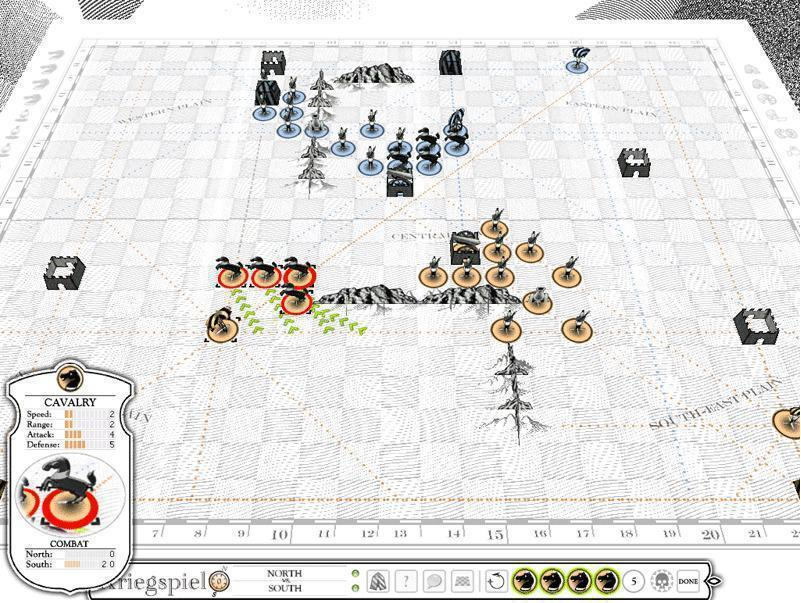
\includegraphics[scale=0.5]{data/kriegspiel.jpeg}
    %Source: \url{https://download.tuxfamily.org/sdtraces/BottinHTML/Bottin_K-O_files/38e33e3e441a297d6fc55b27dd6a98d3.jpeg}
    \caption{Jeu \textit{Kriegspiel} : jeu de pions complexe développé par l'armée du royaume de Prusse au XIXe siècle pour enseigner les tactiques de combat aux officiers, adapte aussi dans des versions plus modernes \cite{livermore1879american}}
\end{figure}

Par exemple, Nous avons trouvé un jeu similaire à notre projet : \textit{Kriegspiel}, un des plus anciens jeux de guerre, datant du XIXe siècle, initialement créé par des généraux Prussiens pour former leurs officiers.

\begin{figure}[H]
    \centering
    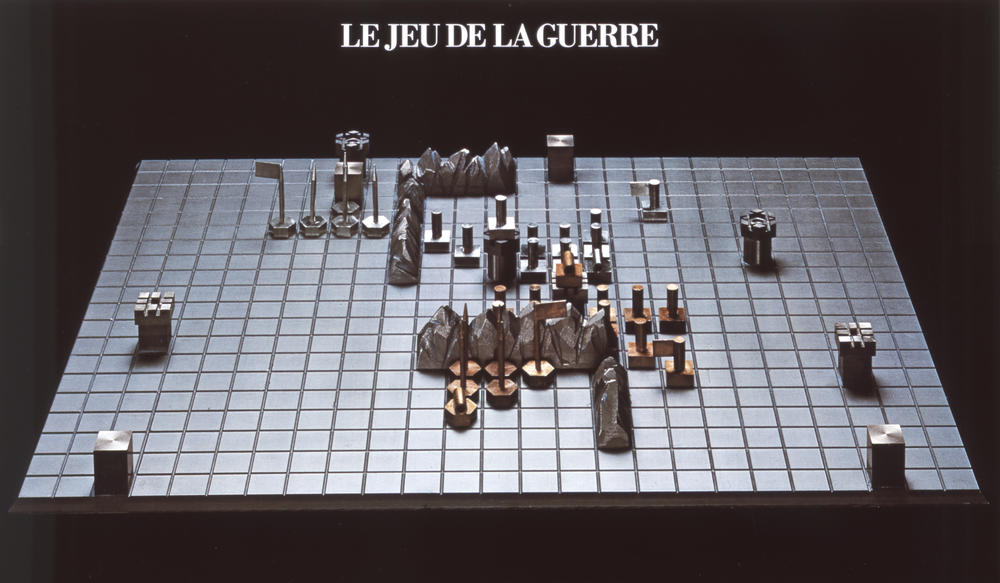
\includegraphics[scale=0.2]{data/Cavalry_at_dusk.jpg}
    \caption{\textit{Le Jeu de la guerre (War Game)} : Plateau du jeu}.
    %source https://upload.wikimedia.org/wikipedia/commons/thumb/f/f9/Cavalry_at_dusk%2C.jpg/250px-Cavalry_at_dusk%2C.jpg
\end{figure}

Le Jeu de la Guerre \cite{frwiki:189457170} est un essai stratégique de Guy Debord et Alice Becker-Ho édité en 1987.
C'est un jeu qui se joue sur un plateau de 25x20. Contrairement à Desert Fox le plateau est en carré. La ressemblance avec Desert Fox est la formation d'unité (infanterie, cavalerie, artillerie).
Le but du jeu, est de vaincre l'adversaire, soit en détruisant son arsenal ou toutes ses unités. À chaque tour, un joueur peut déplacer cinq unités.


\begin{figure}[H]
    \centering
    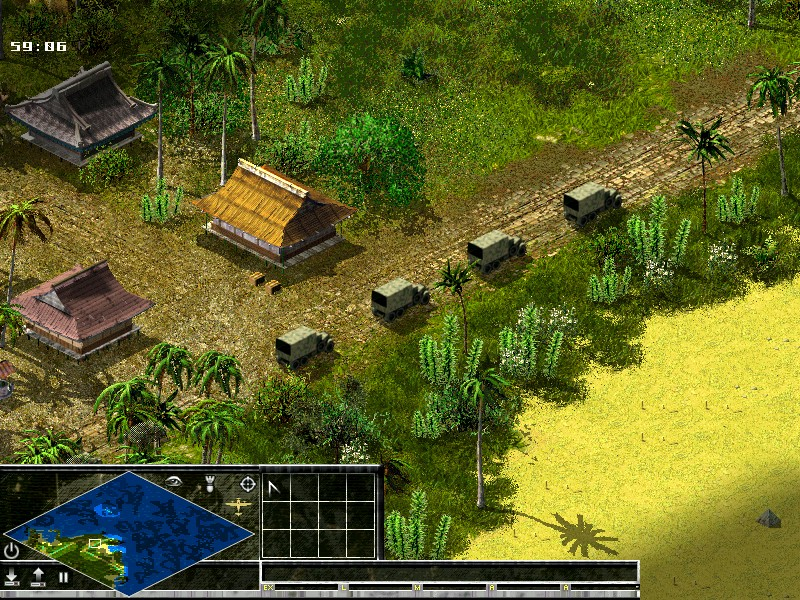
\includegraphics[scale=0.3]{data/sudden_strike_2.jpg}
    %https://cdn.cloudflare.steamstatic.com/steam/apps/612520/ss_e593c9966bc58b7326287db455776b2291718f76.600x338.jpg?t=1644312432
    \caption{\textit{Sudden Strike 2 Gold} : Le jeu propose cinq campagnes, une par faction, composée chacune d’une dizaine de missions : l'URSS, le Japon, l'Allemagne, États-Unis et Royaumes-Unis.}
\end{figure}

Sudden Strike 2 est un jeux-vidéo sortie en 2002. Il s'agit du deuxième volet de la série Sudden Strike. C'est un jeu datant de la seconde guerre mondiale.
Le joueur peut commander les force de l’Allemagne, de l’URSS, du Japon, des États-Unis ou du Royaume-Uni.
Le joueur commence avec un nombre prédéfini d'unités. Ce jeu propose différents scénarios. Plus de 50 unités sont proposées dont : infanterie, char d'assaut, artillerie et aviation.
Il est possible de transporter des troupes, des véhicules et ravitaillements par le train, de mettre en place des ponts aériens ou organiser des opérations de parachute.


\begin{figure}[H]
    \centering
    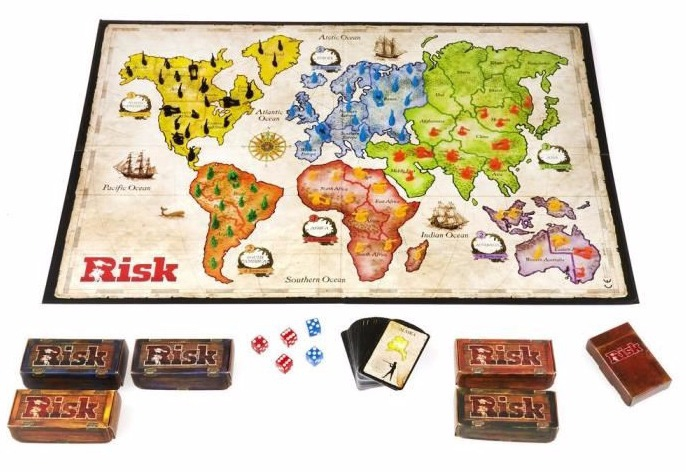
\includegraphics[scale=0.4]{data/risk.jpg}
    \caption{\textit{Risk nouvelle expédition} : Jeu société.}
    % source https://www.espritjeu.com/upload/image/risk-nouvelle-edition-p-image-60508-grande.jpg
\end{figure}
Risk est un jeu de société de guerre. Édité en 1957. Il est possible de jouer de 2 à 6 joueurs. Ce jeu peut durer jusqu'à 2 heures. À la différence des autres jeux, ce jeu se passe dans le monde. Le plateau représente la Terre.
Après la distribution des cartes, tous les joueurs posent un fantassin sur chacun de ces pays, puis le donneur des cartes choisi une mission. Les joueurs doivent deviner la mission des adversaires.
Les joueurs peuvent bluffer.
Le but du jeu est d'allouer des armées dans les territoires contrôlés puis attaquer les zones voisines. Un participant est éliminé s’il ne lui reste plus de territoires.


\begin{figure}[H]
    \centering
    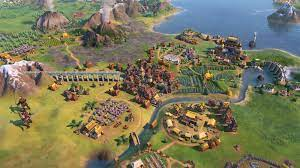
\includegraphics[scale=0.8]{data/civilization.jpeg}
    %source https://www.gamecash.fr/thumbnail-650/civilization-6-2-e146117.jpg
    \caption{\textit{civilization VI} : jeu vidéo.}
\end{figure}
Civilization VI est un jeu vidéo de stratégie. Il s'agit du sixième opus.
Le joueur doit mener sa civilisation à la victoire.
Il peut fonder de nouvelles villes et construire des aménagements ainsi que déclarer la guerre et se procurer un empire tout en défendant le sien.


